\subsection{\textbf{引言:我们是如何从代码到机器人控制的}}
通过之前的学习,相信大家已经对如何再CMake的帮助下使用C++编写代码有了一定的了解。
之后你们会学习一些针对特殊需求的库,比如OpenCV、cuda等。他们能解决一些特定的问题,比如视觉处理
和模型运行等。

在此之前,你们需要学会如何把将要学的这些内容连接起来。比如,机器人的相机、传感器、MCU发来的信息会不断地
想你发送信息,我们需要一种“系统”能够从容地处理这些信息,对这些信息进行运算再发送出去。
这个“系统”其实就是操作系统(OS, Operating System)。对于个人计算机,我们使用的是Windows、Linux、Mac OS等,
他们帮我们进行了很多底层的工作,比如处理硬件、网络、驱动程序等。
而对于机器人来说,我们使用的是\textbf{ROS}(Robot Operating System),它帮助我们管理多个信息来源和不同信息,同时负责不同模块之间的通信。
这样一来,我们就不必要关注多个线程之间的同步、死锁等问题,只需要专注于业务逻辑的实现。
可以理解为如果不使用ROS2,我们需要自己使用C++的多线程库编写一个复杂的多线程系统,而ROS2可以替代你们上一章学的C++多线程,因为一个复多线程系统的编写
往往setTimeOut、wait等操作非常复杂,而ROS2使用DDS(Data Distribution Service)来实现通信,它已经帮我们处理了很多底层的细节。
\subsubsection{ROS2的版本}
和Linux与Ubuntu的关系类似,ROS2也有不同的版本或者说分支,比如ROS2 Foxy、ROS2 Eloquent等。
现在,我们队伍中主流使用的版本是\textbf{ROS2 Humble Hawksbill}。
\begin{figure}
    \centering
    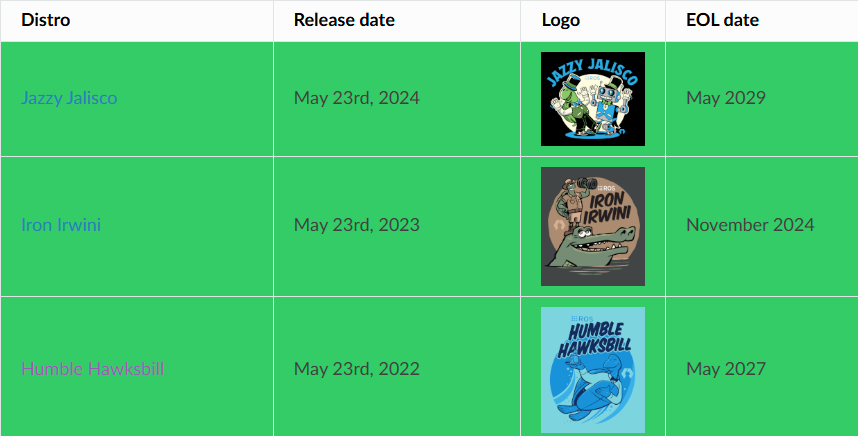
\includegraphics[width=0.8\textwidth]{Chapter4/img/ros2_logo.png}
    \caption{ROS2的最新版本跟新情况}
    \label{fig:ros2_logo}
\end{figure}

\subsubsection{ROS2的安装}

首先,我们需要安装ROS2的Humble Hawksbill 版本。
\begin{tbash}
    wget http://fishros.com/install -O fishros && . fishros
\end{tbash}
这条命令会帮你下载并运行一个脚本,根据它的引导选择下载ROS humble即可。
大概的输出为:
\begin{tbash}
    some output should be here...
\end{tbash}
这是一个非常好用的网站,江湖人称鱼香ROS。

这个命令在配置一个白板的Ubuntu系统时一般第一个运行,它会引导你更换系统源、安装必要的依赖包、配置环境变量等(甚至是下载QQ和微信)
这就减少了去官网上一个个寻找ubuntu版本的麻烦。

\subsection{ROS2架构}
\subsubsection{ROS2的系统架构}
ROS2的系统架构如下图所示:
\begin{figure}[h]
    \centering
    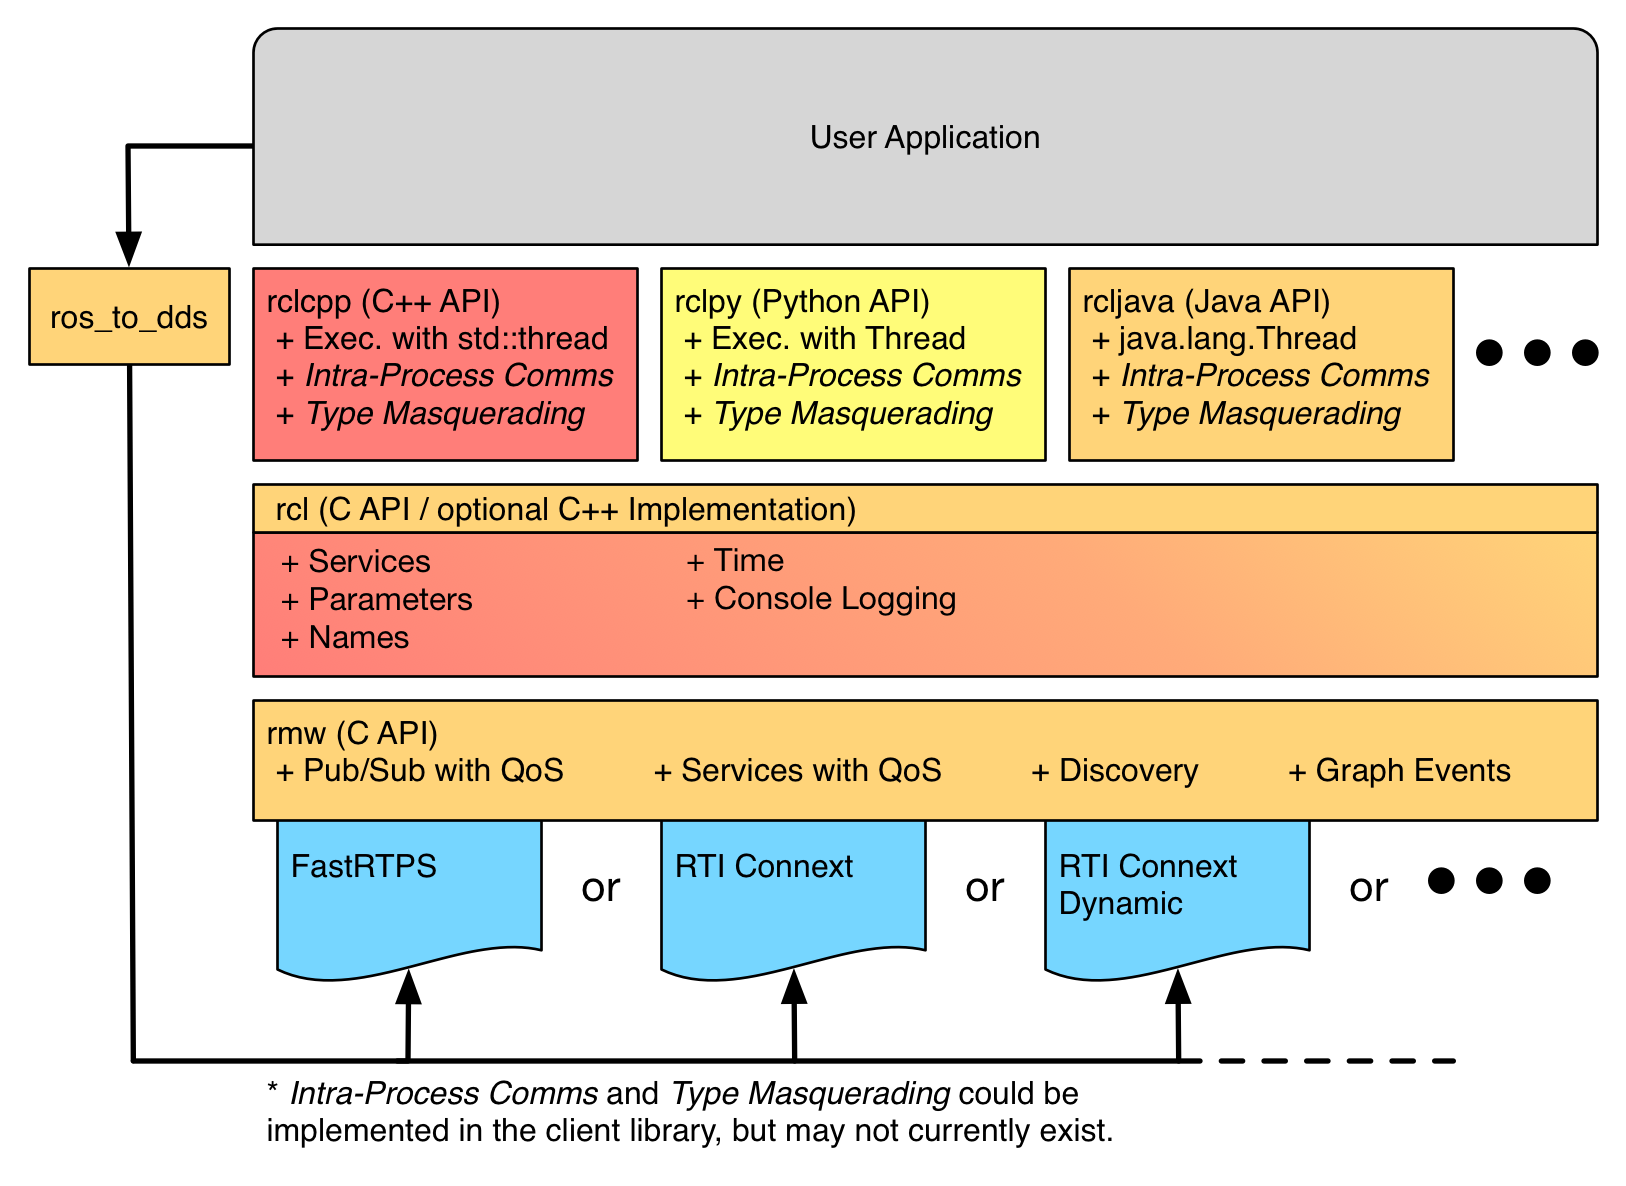
\includegraphics[width=0.8\textwidth]{Chapter4/img/ros2_arch.png}
    \caption{ROS2架构}
    \label{fig:ros2_arch}
    虽然你可能现在看不懂这个图,但不妨等学完之后再回过头来看看。
\end{figure}
一些需要听说过的属于的翻译:
\begin{itemize}
    \item \textbf{rclcpp}: ROS Client Library for C++,它是ROS2的C++客户端库,负责ROS2节点的创建、通信、生命周期管理等,我们使用的主要是这个库。
    \item \textbf{rmw}: ROS Middleware,它是ROS2的中间件,负责底层通信的实现。
    \item \textbf{Qos}: Quality of Service,它是ROS2的通信质量保证机制,用来控制通信的延迟、带宽等。
    \item \textbf{DDS}: Data Distribution Service,它是ROS2的分布式数据服务,用来实现ROS2节点之间的通信。
\end{itemize}
\subsubsection{ROS2的节点与组件}
\textbf{ROS2的基本思想是分布式的、模块化的。}

ROS2的节点是ROS2系统的基本单元,它可以包含多个ROS2组件。

我们可以用这个图来直观地理解ROS2的\textbf{节点}:
\begin{figure}[h]
    \centering
    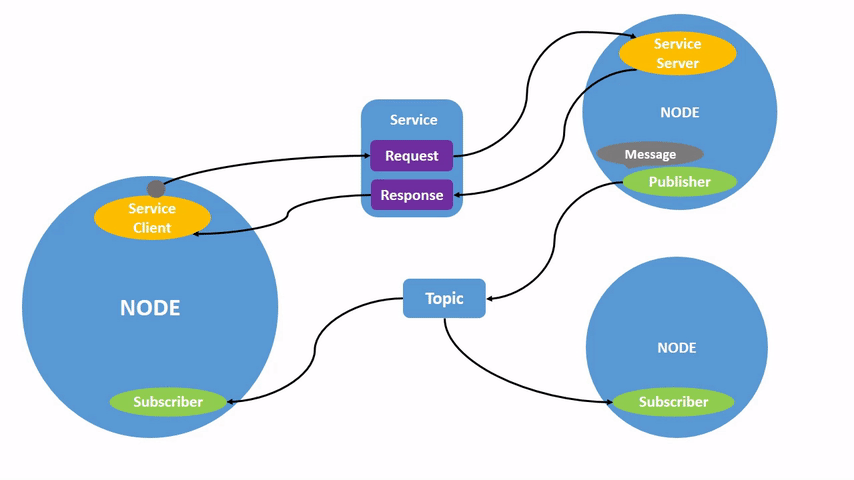
\includegraphics[width=0.8\textwidth]{Chapter4/img/ros2_node.png}
    \caption{ROS2节点与组件}
    \label{fig:ros2_node}
\end{figure}
这是一个动图,你可以去\underline{\href{https://docs.ros.org/en/humble/_images/Nodes-TopicandService.gif}{这里}}播放看看。

这个图直观的反映了ROS2的模块化是依靠\textbf{节点}完成的,节点的职责可以是接收某个传感器的信息(比如相机),也可以是对数据进行处理的流程(比如对相机的图像进行滤波),也可以是提供服务(比如反馈相机的参数信息)
当然这些功能也可以在一个节点中完成。同时可以注意到,节点之间的信息交流是依靠组件(Component)来实现的,一般来说一个节点的运行入口函数也是某个组件的回调函数。


对于我们实际上手操作的情况下,我们更感知的操作方式有两种。
一是使用CLI tools(command-line interface),二是使用Client Libraries。
我们一般使用CLI tools来创建、运行、调试节点,而Client Libraries则用于编写节点的逻辑。

\subsection{使用RCLCPP接口}
由图\ref{fig:ros2_arch}可以看到,rclcpp是ROS2的C++接口,我们在C++中使用这个来描述机器人的节点和节点之间的行为。
\subsubsection{创建ROS2工作空间和第一个包}
首先,你需要寻找一个你喜欢的地方新建一个文件夹,这个名字不重要,但建议起个有意义的名字。
\begin{tbash}
    mkdir -p ~/ros2_ws/src
    cd ~/ros2_ws/src
\end{tbash}

这里把工作空间(就是文件夹)命名为ros2\_ws,并在其下创建了一个src文件夹,这个文件夹是ROS2的源代码存放的地方。

接着,我们需要创建一个ROS2包,这个包就是我们要编写的节点。
\begin{tbash}
    ros2 pkg create --build-type ament_cmake my_package
\end{tbash}
此时的文件目录应该为:
\begin{figure}
    \centering
    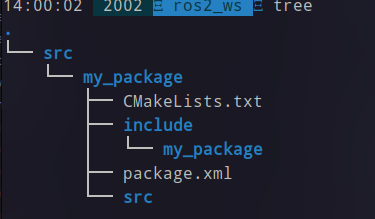
\includegraphics{Chapter4/img/treeofws.png}
    \label{fig:treeofws}
\end{figure}

然后回到工作空间的根目录(ros2\_ws),输入以下命令编译这个包:

\begin{tbash}
    colcon build
\end{tbash}

编译好的包会产生,build、install、log三个文件夹,其中build文件夹是编译好的可执行文件,install文件夹是编译好的库文件,log文件夹是编译过程的日志。

除此之外,我们还有有一个神秘小工具介绍一下。一般来说,如果按照普通的编写流程,在ros2的包中链接一个库会有多步操作,但是如果使用ament\_cmake\_auto,就可以一步到位。
我们只需要将CMakeLists.txt文件改为\ref{lst:ament_cmake_auto_config}。之后再加入库的依赖关系,至于需要在xml文件中添加depend命令就可以,就可以自动下载、编译、链接库。
可以参考\url{https://zhuanlan.zhihu.com/p/438191834}

之后我们就可以开始编写代码了。
\subsubsection{编写第一个ROS2节点}

新建my\_node.cpp和my\_node.h文件。并在这两个文件中新建一个类my\_node,继承自rclcpp::Node。
Node类是ROS2提供的基础的类,我们会在这个基类上进行扩展。

其构造函数一般是用来设置节点的发布者和订阅者,绑定对应的回调函数。实现为代码\ref{lst:my_node_cpp}(其实这个数字可以点击)的3-38行。
\subsubsection{编写发布者和订阅者}
要编写发布者和订阅者,我们需要使用rclcpp::Publisher和rclcpp::Subscription。
现在节点的类中定义一个私有成员变量,用来保存订阅者的句柄,并在构造函数中初始化。
需要注意,定义的应该是$rclcpp::Publisher<T>::SharedPtr/create\_subscription<T>::SharedPtr$即共享指针,

初始化的时候需要使用$create\_publisher<T>/create\_subscription<T>$这个模版函数,它传入的模版参数是消息类型,函数参数是topic名称、QoS等(这个等一般是指的一个回调函数的函数指针)。


\begin{tcode}
    string_publisher_ = create_publisher<std_msgs::msg::String>(
         "send",
         10
         );
\end{tcode}
这个代码将类的成员变量string\_publisher\_绑定到话题名称为"send"的发布者,QoS为10。这个话题名称是我随便起的,
QoS是Quality of Service的缩写,用来控制发布者和订阅者之间的通信质量,一般来说基本的数据通讯用$1$,图像用$10$,当然也有更高级的办法确定通讯质量。

这样变量string\_publisher\_所指的空间就有了一个发布者,他会发布std\_msgs::msg::String类型的消息。但是很明显你能发现他并不会发布消息,因为还没有编写发布消息的逻辑。
不妨在订阅回调中进行发布。

\begin{tcode}
    string_subscription_ = create_subscription<std_msgs::msg::String>(
         "receive",
         10,
         std::bind(&my_node::subscription_callback, this, std::placeholders::_1)
         );
\end{tcode}
这个代码将类的成员变量string\_subscription\_绑定到话题名称为"receive"的订阅者,QoS为10。
std::bind其实在C++11之后已经可以被lambda函数平替了,但是某些时候会报神秘段错误,所以这里还是使用bind来绑定一个成员函数。(这里相当于$[this] \{ timer\_callback(); \}$)
this是所有类的成员函数的第一个参数(这个知识应该不冷门吧),用来绑定当前类的实例,$std::placeholders::_1$是C++的占位符,用来指第一个参数,也就是收到的消息。
这个绑定的成员函数就是所谓的订阅回调函数,他会在收到消息时被调用。然后就可以在这个函数中写收到信息之后要干什么了。
\begin{tcode}
void my_node::subscription_callback(const std_msgs::msg::String::SharedPtr msg)
{
 RCLCPP_INFO(get_logger(), "I hear %s", msg->data.c_str());
 auto message = std_msgs::msg::String();
 message.data = "I can hear:" + msg->data;
 string_publisher_->publish(message);
}
\end{tcode}

函数体中第一行是通过RCLCPP的日志系统打印收到的消息。RCLCPP的日志系统可以输出以下几种信息:
\begin{itemize}
    \item RCLCPP\_INFO: 一般用于输出一些信息,比如发布者发布消息、订阅者收到消息等。
    \item RCLCPP\_WARN: 一般用于输出一些警告信息,比如有一些错误发生。
    \item RCLCPP\_ERROR: 一般用于输出一些错误信息,比如有一些不可预料的错误发生。
    \item RCLCPP\_FATAL: 一般用于输出一些致命错误信息,比如程序崩溃了。
\end{itemize}
这些消息一方面打印在终端之外,另一方面也会被ROS2的日志系统记录下来,方便后续分析。

之后的三行是创建一个String消息类型,并设置它的data字段为收到的消息加上一段文字。然后使用刚刚定义的发布者发布这个消息。

这样我们就完成了一个最简单的ROS2节点,它可以发布和订阅消息,并且可以处理收到的消息。
下面是检验这个节点是否能正常工作,对于写代码的时候,我们直接可以用IDE的运行功能来测试。
正式一点来说(比如在实车测试的时候),我们需要在终端中工作空间下,输入以下命令:
\begin{tbash}
    colcon build
    ros2 run my_package my_node
\end{tbash}
然后打开rqt的Message Publisher和Message Monitor,分别订阅和发布话题,可以查看节点的运行情况。
经过一番设置之后,我们就可以看到:
\begin{figure}[h]
    \centering
    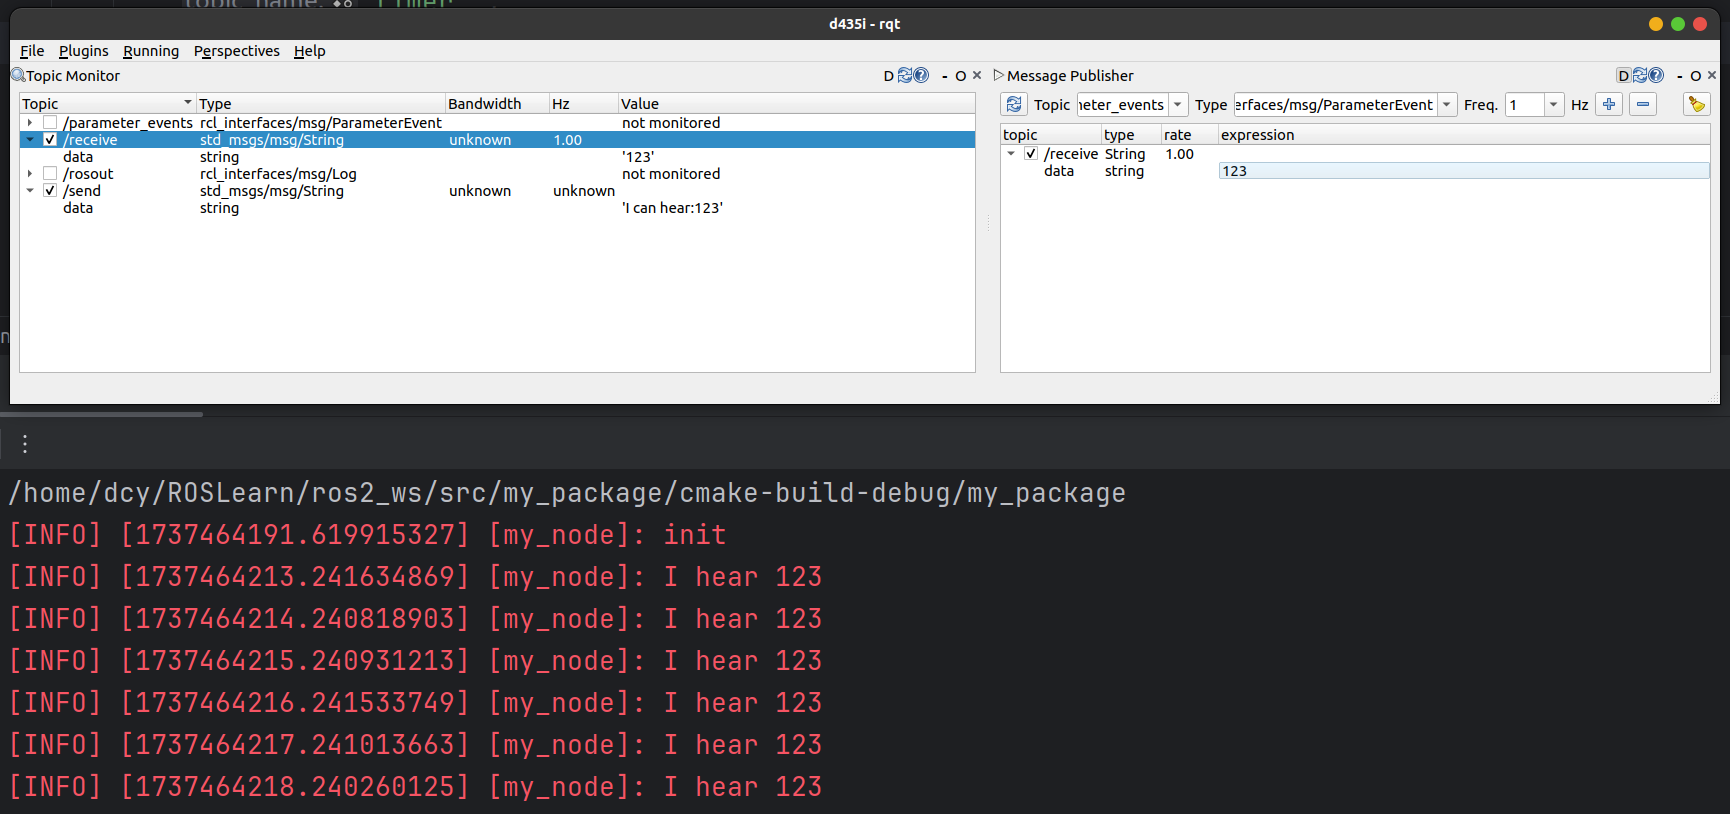
\includegraphics[width=0.8\textwidth]{Chapter4/img/rqt_vision.png}
    \caption{用rqt看节点运行情况}
\end{figure}

顺带一提,这前面的一长串数字是时间戳,用来记录消息的发布时间,这个时间是从Linux内核中以1970年1月1日午夜(00:00:00)为基准的系统时间,这个基准是C语言time
\begin{tcode}
    1969年8月,贝尔实验室的程序员肯汤普逊利用妻儿离开一个月的机会,

    开始着手创造一个全新的革命性的操作系统,
    
    他使用B编译语言在老旧的PDP-7机器上开发出了Unix的一个版本。

    随后,汤普逊和同事丹尼斯里奇改进了B语言,
    
    开发出了C语言,重写了UNIX,新版于1971年发布。

    那时的计算机操作系统是32位,时间用32位有符号数表示,则可表示 68 年,

    用32位无符号数表示,可表示136年。他们认为以1970年为时间原点足够可以了。 

    因此,C 的 time 函数 就这么 定了,后来的 java 等也用它,
    
    微机也用它,工作站本来就是unix系统当然也用它。
    
    (今后若用64位机年限更没问题。)

    1970年1月1日 算 UNIX 和 C语言 生日。
\end{tcode}

\subsubsection{定时器回调}
这个非常简单,定义RCLCPP的TimeBase类型,然后用C++中的$chrono$库来提供定时器时间,再使用$create_wall_timer$绑定一个函数作为回调函数即可。
\begin{tcode}
    //定义成员变量
    rclcpp::TimerBase::SharedPtr timer_;
    //构造函数
    timer_ = create_wall_timer(
        std::chrono::milliseconds(1000), // 定时器间隔
        std::bind(&my_node::timer_callback, this)); // 回调函数
    //回调函数
    void my_node::timer_callback()
    {
        RCLCPP_INFO(get_logger(), "%d s", ++cnt_);
        auto time_msg = std_msgs::msg::String();
        time_msg.data = "Now is " + std::to_string(cnt_);
        timer_publisher_->publish(time_msg);
    }
\end{tcode}
这个回调函数是每秒钟被调用一次,打印一下计数器的值,并发布一个计数器的消息。

\subsubsection{编写自定义消息类型}
所谓自定义消息类型,就是使用基本的数据类型加上ros2中$std_msgs$或$sensor_msgs$等消息包中的消息类型,来定义我们自己的消息类型。
以实际应用例子,我们的机器人在自瞄时传输瞄准的装甲板数据时,需要知道id(地方装甲板的编号),yaw(装甲板的偏航角度)等信息。
同时我们还要知道识别到的时间信息等,所以只有自定义消息类型才能满足需求。


在ROS 2中,使用RCLCPP接口创建自定义消息类型需要以下步骤:

1. 创建自定义消息包

首先,创建一个专门用于存放自定义消息的包。例如,创建一个名为my\_msgs的包:
\begin{tbash}
    ros2 pkg create --build-type ament_cmake my_msgs
\end{tbash}

然后在该包中创建msg目录,用于存放自定义消息文件。

\textbf{消息包名必须大写字母开头,只包含数字和字母,内容中不能有大写字母。}

2. 定义自定义消息

在msg目录中创建.msg文件,定义消息的结构。
\begin{tbash}
    std_msgs/Header header
    uint8 id
    float64 yaw
    bool detect_success
\end{tbash}

3. 修改CMakeLists.txt文件和package.xml文件

建议直接看附录代码\ref{lst:xml_2}

4. 编译自定义消息
在工作空间中运行以下命令以编译自定义消息:
\begin{tbash}
    colcon build --packages-select my_msgs
    source install/setup.bash
\end{tbash}

编译完成后,自定义消息的C++头文件将生成在install/my\_msgs/include/my\_msgs/msg目录下。

5. 在节点中使用自定义消息

在其他节点中使用自定义消息时,需要在CMakeLists.txt中添加对my\_msgs的依赖,并在代码中包含自定义消息的头文件。例如:
就像其他ROS2自带的消息类型一样。

\subsubsection{ROS2的消息类型}

1.std\_msgs
\begin{figure}[h]
    \centering
    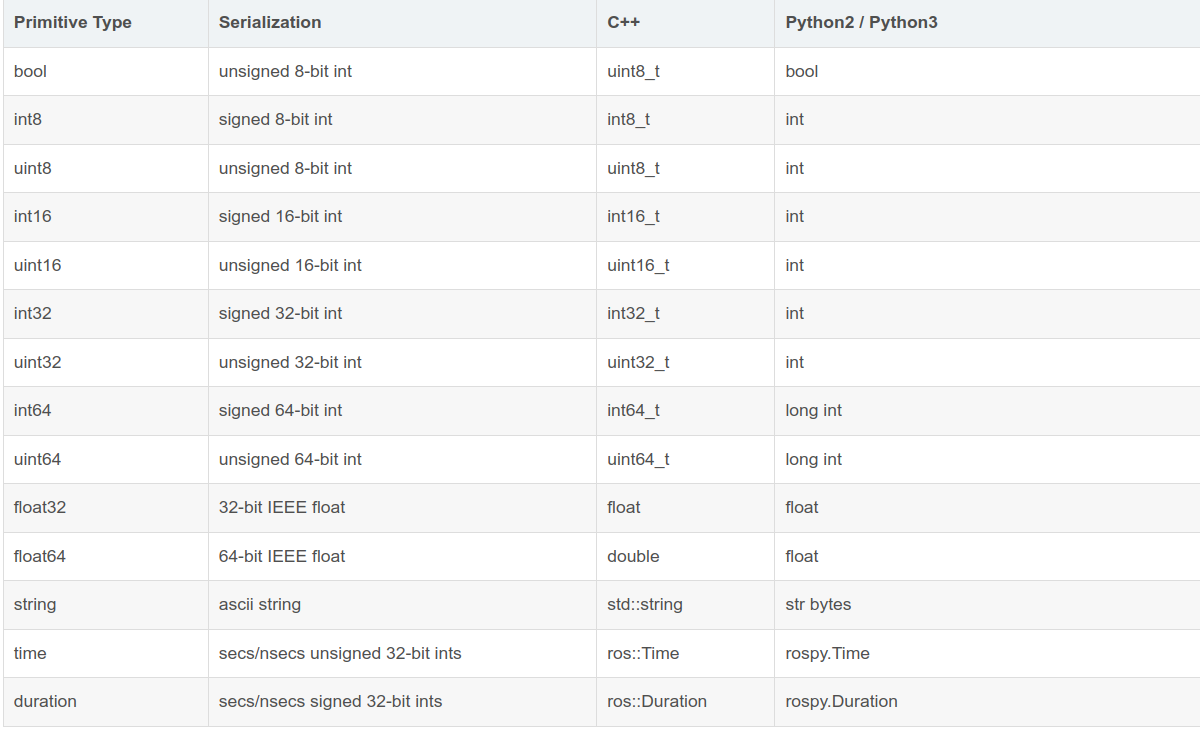
\includegraphics[width=0.8\textwidth]{Chapter4/img/ros_message1.png}
    \caption{std\_msgs的变量}
\end{figure}
\begin{figure}[h]
    \centering
    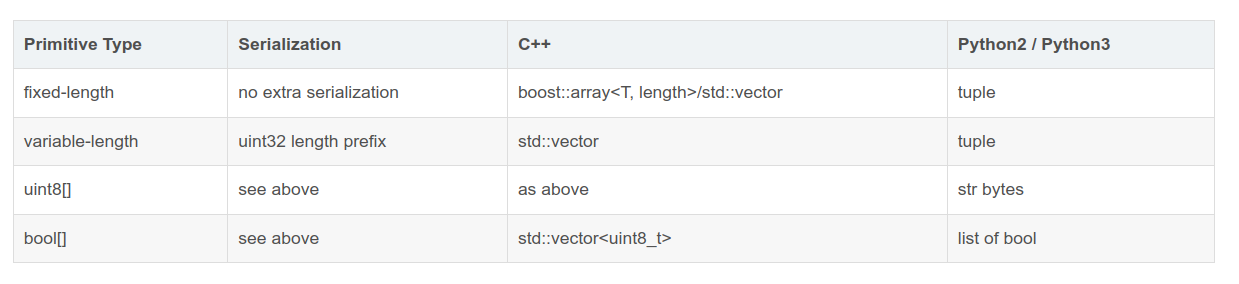
\includegraphics[width=0.8\textwidth]{Chapter4/img/ros_message2.png}
    \caption{std\_msgs的数组}
\end{figure}


\begin{center}
    \begin{tabular}{lll}
        \hline
        &std\_msgs::Header是标准消息头& \\
        \hline
        time & stamp & 时间戳 \\
        string & frame\_id & 用于标识坐标系 \\
        \hline
    \end{tabular}
\end{center}

处理std\_msgs之外,还有comm\_msgs,包括:actionlib\_msgs、diagnostic\_msgs、geometry\_msgs、nav\_msgs、sensor\_msgs

2.geometry\_msgs。最常用的几何消息类型,定义了描述机器人状态的各种类型,比如点、速度、加速度、位姿等。

Vector3(三个float64)可以传输三维坐标,Vector3Stamped(带时间戳的三维坐标)可以传输带时间戳的三维坐标。
Quaternion、QuaternionStamped是传输四元数的消息类型。
Transform、TransformStamped是传输坐标系变换关系的消息类型。

3.sensor\_msgs。包含了传感器数据,包括图像、激光、雷达、IMU等。

主要用的就上面三种消息类型。

\dots \dots \dots
Qos: 
更多更详细内容请参考官方文档。

\subsection{提升内容}
这部分是一些ROS2的较高级内容,主要是介绍名字和基本用途。(主要是有的我也不熟)
可以在需要的时候查找对应关键词。

\textbf{功能:}
\begin{enumerate}
    \item ROS2 launch,可以用来启动多个节点,并设置参数。用于启动复杂的系统。
    \item service的代码实现
    \item ROS2参数,可以通过launch文件设置参数,也可以在代码中设置参数。
    \item rosbag 用于记录和重放ROS2的消息。这点对于调试和分析非常有用,可以做到在家就能调试。
    \item 通过ROS2组件的形式启动ROS2节点。
\end{enumerate}

\textbf{包:}
\begin{enumerate}
    \item cv\_bridge 包,用于ROS2和OpenCV之间的互相转换。
    \item tf2 包,提供了一个坐标变换的框架。
    \item rviz 包,用于可视化ROS2的消息。(或者用foxglove studio)
    \item moveit2 包,用于机械臂控制。
    \item navigation2 包,用于导航。
    \item fmt 包,可以自定义打印日志的格式。
\end{enumerate}